\documentclass[border=10pt]{standalone}
\usepackage{tikz}\usepackage{amsmath}\usetikzlibrary{arrows.meta}
\begin{document}
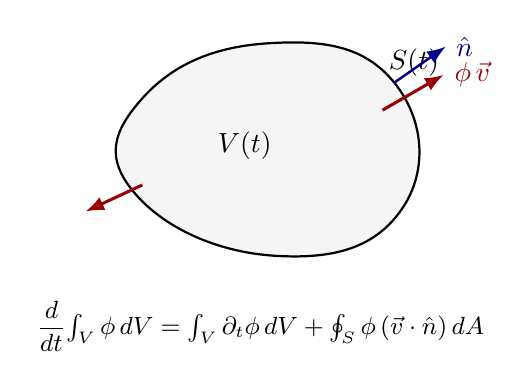
\begin{tikzpicture}[line width=0.9pt,>={Latex[length=2.4mm]}]
  \draw[thick,fill=black!4] plot[smooth cycle,tension=0.8] coordinates {(-1.5,0.7)(0.1,1.4)(1.7,0.9)(1.8,-0.7)(0.2,-1.3)(-1.6,-0.5)};
  \node at (-0.2,0.1){$V(t)$};
  \node at (1.95,1.15){$S(t)$};
  % normal y flujo phi v
  \draw[->,blue!55!black] (1.7,0.9)--++(35:0.8) node[right]{$\hat n$};
  \draw[->,red!60!black,line width=1.1pt] (1.55,0.55)--++(30:0.9) node[right]{$\phi\,\vec v$};
  \draw[->,red!60!black,line width=1.1pt] (-1.5,-0.4)--++(205:0.8);
  \node at (0,-2.2){\small $\dfrac{d}{dt}\!\int_{V}\phi\,dV=\int_V\partial_t\phi\,dV+\oint_S\phi\,(\vec v\cdot\hat n)\,dA$};
\end{tikzpicture}
\end{document}
